\documentclass[3p]{elsarticle} %preprint/3p

\usepackage{hyperref}

\journal{ }

\usepackage{amsmath} %added for maths environments (equation and align)
\usepackage{amssymb}
\usepackage{upgreek}
\usepackage{bm} %bold symbols by using \bm
\usepackage{mathtools, nccmath} %added for \xrightleftharpoons

\usepackage{subcaption} %allowing for subcaptions and subfigures
\captionsetup[sub]{font=normalsize}%normalsize

\usepackage{algorithm} %added for algorithm box
\usepackage{algpseudocode}

\usepackage[autostyle]{csquotes}
\MakeOuterQuote{"}

\bibliographystyle{elsarticle-num}

% slightly altering rules for figure placement to prevent full-page figures
\usepackage{placeins}
\renewcommand{\floatpagefraction}{.90}
\renewcommand{\topfraction}{.90}

\usepackage[capitalise, nameinlink]{cleveref}

\usepackage{todonotes} %added for todo notes
\let\oldtodo\todo
\renewcommand{\todo}[1]{\oldtodo[inline]{#1}}
%\renewcommand{\todo}[1]{\oldtodo[color=white!40,inline]{#1}}
\newcommand{\toask}[1]{\oldtodo[color=green!40, inline]{#1}}
\newcommand{\wrn}[1]{\oldtodo[color=red!40, inline]{#1}}

\usepackage{xcolor}
\usepackage{listings}
\usepackage{lstautogobble}
\usepackage[numbered]{matlab-prettifier}
\lstdefinestyle{mystyle}{
	numbers=left,
	numberstyle=\footnotesize,
	numbersep=8pt,
	style=Matlab-editor,
	tabsize=4,
	basicstyle=\ttfamily\footnotesize,
	numbersep=12pt,
	frame=none,
	autogobble=true
}

\newcommand{\citeMe}{\href{https://doi.org/10.1016/j.cma.2023.116235}{T Hageman, JZ Mejia,R Duddu, and E {Martinez-Pa{\~n}eda}. \textit{Ice Viscosity Governs Hydraulic Fracture Causing Rapid Drainage of Supraglacial Lakes}. The cryosphere} \citep{Hageman}}

\begin{document}

\begin{frontmatter}
\title{IceHydroFrac: A MATLAB code to simulate water-filled crevasse propagation and uplifting of ice sheets }

\author[1]{Tim Hageman \corref{mycorrespondingauthor}}
\cortext[mycorrespondingauthor]{Corresponding author}
\ead{tim.hageman@eng.ox.ac.uk}
\author[2]{Jessica Mejía}
\author[3]{Ravindra Duddu} 
\author[1]{Emilio Martínez-Pañeda}

\address[1]{Department of Engineering Science, University of Oxford, Oxford OX1 3PJ, UK}
\address[2]{Department of Geology, University at Buffalo, Buffalo, NY 14260, USA}
\address[3]{Department of Civil and Environmental Engineering, Department of Earth and Environmental Sciences, Vanderbilt University, Nashville, TN 37235, USA}

\begin{abstract}
Documentation that accompanies the \textit{MATLAB} code \href{https://github.com/T-Hageman/MATLAB_IceHydroFrac}{IceHydroFrac, available from \textcolor{blue}{here}}. This documentation explains the usage of the implemented finite element framework, and highlight the main files.  

If using this module, please cite: \citeMe{}.
\end{abstract}

\begin{keyword}
MATLAB, Hydraulic fracture, Greenland Ice Sheet, Crevasse, Numerical simulation, Viscous effects
\end{keyword}

\end{frontmatter}

\begin{figure}
	\centering
	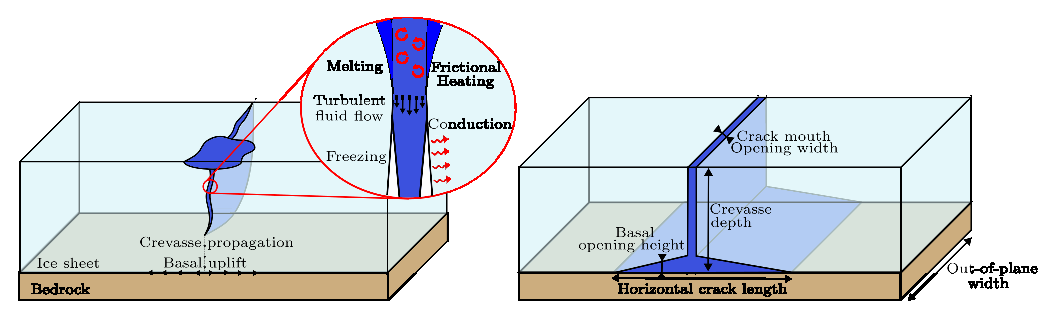
\includegraphics[width=16cm]{Figures/CaseOverview.eps}
	\caption{Overview of the system simulated using the presented MATLAB code}
\end{figure}

\newpage
\tableofcontents

\newpage
\section{Introduction}
\todo{Intro sentences}

\subsection{Basic usage}
All parameters are set within and relevant functions are called from the matlab file "main.m", and running this file performs the full simulation. Parameters are also set within this file, for instance defining the visco-plastic model through:
\lstinputlisting[firstnumber=64,firstline=64,lastline=73,style=mystyle,title=main.m]{../main.m}
These parameters are automatically passed along to the relevant physics models once they are initialized. As such, no changes in other files are needed to adapt the simulation set-up for other parameters. 

\section{Summary of included files}
The code is set up in a object-oriented manner, defining matlab classes for each sub-component and providing their accompanying methods. As a result, a clear distinction is made between different components, and each can be used and altered with limited/no impact on other components. Here, the different classes are described. The commenting style employed within the code is compatible with the matlab help function, as such information about all usable methods within a class can be accessed by including the relevant folders, and typing, for instance, "help Solver" to print all variables contained within and all function available from the solver. 

\subsection{main.m}
This is the main file, from which all classes are constructed and the actual simulation is performed. Within it, all properties used within other classes are defined as inputs. These properties are then passed on to initialize the "physics" object, via 
\lstinputlisting[firstnumber=147,firstline=147,lastline=148,style=mystyle,title=main.m]{../main.m}
taking all relevant input parameters within the physics\_ in structure, and an initial time step increment dt0. In a similar manner, the mesh is also initialized from a structure of properties, 
\lstinputlisting[firstnumber=142,firstline=142,lastline=145,style=mystyle]{../main.m}
which reads the mesh from a file, initializes the required elements and node groups, displays the mesh in  a figure, and confirms the mesh is valid and prints statistics related to the area of each separate element group to the output. Finally, the main file performs the time-stepping, calling the function:
\lstinputlisting[firstnumber=195,firstline=195,lastline=196,style=mystyle]{../main.m}
to solve the actual time increments. 

After each time increment, outputs are saved into a single structure for later plotting, 
\lstinputlisting[firstnumber=198,firstline=198,lastline=208,style=mystyle]{../main.m}
These outputs are:
\begin{enumerate}
  \setcounter{enumi}{199}
  \item tvec: This contains all time increments at which the other elements within this structure have outputted data. Notably, as the time increment varies between the initialization period ($tvec(i)<0$) and actual simulations ($tvec(i)\geq 0$) differs, this vector is also required to translate the number of the time step (as used within the naming of full output files) to the actual time of the outputs.
  \item Lfrac: This is the length all fractured interfaces. When the crevasse has yet to reach the base, this corresponds to the depth of the crevasse. After reaching the bottom, this is the depth of the crevasse (=the ice thickness) plus the total length of the horizontal cracks (both directions summed together).
  \item Qvec: This reports the total thermal energies produced/consumed throughout the simulation. The first element of this vector corresponds to the thermal energy conducted into the ice, the second to the heat produced by the turbulent flow due to friction, and the final element corresponds to the thermal energy used to cause freezing/melting of the crevasse walls. These values are the integrated totals for the complete crack, and are also integrated over the complete time. 
  \item Qinflow: The total volume of fluid that has entered the crevasse from the inlet at the surface. As with all other outputs, this is given per metre of unit depth.  
  \item qCurrent: The current fluid inflow at the top inlet, $\partial \text{Qinflow}/\partial t$.
  \item upLift: Surface displacement at the centre of the top surface, coinciding with the crevasse. This contains the horizontal displacement (half the crevasse opening height), and the vertical displacement.
  \setcounter{enumi}{206}
  \item SurfaceDisp: Vectors containing horizontal and vertical displacements for the complete top surface of the ice-sheet. The coordinates that correspond to the given data points are saved within TimeSeries.SurfaceCoords. 
\end{enumerate}
In addition to these time series, full outputs are saved after every 10 time steps, 
\lstinputlisting[firstnumber=215,firstline=215,lastline=219,style=mystyle]{../main.m}
These output files are appended with the number of the time increment during which the output is saved, and they contain all information required to restart a previously interrupted simulation. 

\subsection{Models}


\subsubsection{BaseModel}



\subsubsection{Constrainer}



\section{Sample results}


\bibliography{references}

\end{document}
